\documentclass[t]{beamer}
\usepackage{CJKutf8}
\usepackage{amsfonts}
    \usepackage{amsmath}
    \usepackage{amssymb}
    \usepackage{amsthm}
    \usepackage{enumerate}
    \usepackage{graphicx}
    \usepackage{layout}
    \usepackage{mathrsfs}
    \usepackage{fancyhdr}
    \usepackage{subfigure}
    \usepackage{tcolorbox}
    \usepackage{tikz-cd}
    \usepackage{color}
    \usepackage{pifont}
    \usepackage{verbatim}
    \usepackage{mathtools}
    \usepackage{float}
    \usepackage{bm}
    \usetheme{AnnArbor}
% \usetheme{Antibes}
\usecolortheme{beaver}
\usepackage{listings}

% 设置JSON样式
\lstdefinestyle{json}{
    basicstyle=\tiny\ttfamily,
    columns=fullflexible,
    showstringspaces=false,
    commentstyle=\color{gray},
    keywordstyle=\color{blue},
    stringstyle=\color{red},
    breaklines=true,
    frame=single,
    captionpos=b,
    aboveskip=10pt,
    belowskip=10pt
}

\lstset{
    language=Python, % 设置代码块语言为Python
    breaklines=true, % 自动换行
    basicstyle=\small\ttfamily, % 设置基本字体样式
    keywordstyle=\bfseries\color{blue}, % 设置关键字样式
    commentstyle=\itshape\color{gray}, % 设置注释样式
    showstringspaces=false, % 不显示字符串中的空格
    frame=single, % 设置代码块边框样式
    numbers=left, % 行号显示在左侧
    numberstyle=\tiny\color{gray}, % 设置行号样式
    stepnumber=1, % 设置行号间隔
    tabsize=4 % 设置制表符宽度
}


% 设置shell样式
\lstdefinestyle{shell}{
    language=bash,
    basicstyle=\tiny\ttfamily,
    columns=fullflexible,
    showstringspaces=false,
    commentstyle=\color{gray},
    keywordstyle=\color{blue},
    stringstyle=\color{red},
    breaklines=true,
    frame=single,
    captionpos=b,
    aboveskip=10pt,
    belowskip=10pt
}

% 添加网址的命令
\usepackage{hyperref}
% 这是一个带链接文本的示例:\href{https://www.example.com}{点击这里访问网站}
% 普通的示例:\url{https://www.example.com}
% 表格
\usepackage{booktabs}
\usepackage{multirow}

% \setbeamertemplate{navigation symbols}{}

\usepackage{textpos}

\newcommand{\dif}{\mathrm{d}}
\newtheorem{thm}{{定理}}

% some common command
\newcommand{\mm}[1]{$ #1$\newline}
% \newcommand{\tuichu}{\Rightarrow}
% \newcommand{\li}[1]{\newline#1}



\newcommand{\analysis}[2]{\forall \mathcal{E}{#1},\exists \delta {#2},s.t.}
\newcommand{\denyanalysis}[2]{\exists \mathcal{E}{#1},\forall \delta {#2},s.t.}
\newcommand{\yield}{\Rightarrow }
\newcommand{\jj}{\newline}
\newcommand{\ff}[1]{$ #1$}   % math environment + newline
\newcommand{\fgn}[1]{\begin{equation}#1\end{equation}  }
\newcommand{\fg}[1]{$$ #1$$}   % math environment + newline 
\newcommand{\pf}{$proof.$\newline}
\newcommand{\ee}{\newline\ff{\Box}\newline}
\newcommand{\fenshi}[2]{\ff{\frac{#1}{#2}}}
\newcommand{\shenlue}{\vdots\jj}
\newcommand{\abs}[1]{{\left \lvert #1 \right\rvert}}
\newcommand{\loge}[1]{In ({#1})}
\newcommand{\logical}[2]{log_{#2}^{#1}}
\newcommand{\summary}[3]{$\sum_{{#1}={#2}}^{#3}  $}
\newcommand{\denjia}[2]{{#1}\Leftrightarrow {#2}}
\newcommand{\jihe}[3]{ {#1}  = \{ {#2} \mid {#3} \} }
\newcommand{\ve}[2]{\left\langle {#1},{#2}\right \rangle}
\newcommand{\dakuohao}[2]{\begin{array}{rcl}{#1}\end{array} \} \Rightarrow{#2}}
\newcommand{\sxb}[3]{#1^{#2}_{#3}}
\newcommand{\sss}[2]{#1^{#2}}
\newcommand{\xxx}[2]{#1_{#2}}
\newcommand{\bri}[1]{\uppercase\expandafter{\romannumeral#1}}
\newcommand{\ri}[1]{\romannumeral#1} 
\newcommand{\polynomial}[8]{#1_{#2}#6^{#7}+#1_{#3}#6^{#8}+...+#1_{#4}#6+#1_{#5} }
\newcommand{\newd}[4]{f[{#1}_{#2},{#4},{#1}_{#3}]}
\newcommand{\lb}[2]{\begin{align*}\begin{split}{#1}\{ {#2}\end{split}\end{align*}}
\newcommand{\tab}[1]{\begin{array}{ll} {#1}\end{array}}


% 向量乘积
\newcommand{\avg}[1]{\left\langle #1 \right\rangle}
% 偏微分方程
\newcommand{\difFrac}[2]{\frac{\dif #1}{\dif #2}}
\newcommand{\pdfrac}[2]{\frac{\partial{#1}}{\partial{#2}}}
% 不同章节
\newcommand{\one}[1]{\section{#1}}
\newcommand{\two}[1]{\subsection{#1}}
\newcommand{\three}[1]{\subsubsection{#1}}
\newcommand{\aone}[1]{\section*{#1}}
\newcommand{\atwo}[1]{\subsection*{#1}}
\newcommand{\athree}[1]{\subsubsection*{#1}}
% 大括号,左右都有
\newcommand{\lbra}[1]{\left\{  {\begin{matrix} #1 \end{matrix}}\right. } 
% 样式 括号前缀 + 括号 
\newcommand{\lbras}[2]{{#1}\left\{ {  {\begin{matrix} #2 \end{matrix}}}\right. } 
\newcommand{\rbra}[1]{ \left.  {\begin{matrix} #1 \end{matrix}} \right\}  } 
% 模长
\newcommand{\distance}[1]{\parallel #1\parallel }
% 等价
\newcommand{\equ}{\Longleftrightarrow }
% 共轭
\newcommand{\cja}[1]{\overline{#1}}
% 两个矩阵,上面是 方框[] 下面是线条| 中间是 无
\newcommand{\mtx}[1]{\begin{matrix}#1\end{matrix} }
\newcommand{\bmtx}[1]{\begin{bmatrix}#1\end{bmatrix} }
\newcommand{\vmtx}[1]{\begin{vmatrix}#1\end{vmatrix} }
% \newcommand{\table}[1]{\begin{array}[lr]{ccc} #1 \end{array}}

%输入普通字符
\newcommand{\ww}[1]{\text{#1}}

% 所有内容 直接头文件搞定
\newcommand{\everything}[1]{\begin{document}\begin{CJK*}{UTF8}{gkai}#1\end{CJK*}\end{document}}


% 存放代码(失败了)
\newcommand{\cccode}[1]{\begin{lstlisting}#1\end{lstlisting}}

% 改变特定行序列
\newcommand{\ttt}{\subsection{}}

% 嵌套序号
\newcommand{\eee}[1]{\begin{enumerate}#1\end{enumerate}}


% 模板里面的一些宏
\newcommand{\pdfFrac}[2]{\frac{\partial #1}{\partial #2}}
\newcommand{\OFL}{\mathrm{OFL}}
\newcommand{\UFL}{\mathrm{UFL}}
\newcommand{\fl}{\mathrm{fl}}
\newcommand{\op}{\odot}
\newcommand{\Eabs}{E_{\mathrm{abs}}}
\newcommand{\Erel}{E_{\mathrm{rel}}}
% 变化颜色
\newcommand{\red}{\textcolor{red}}
\newcommand{\blue}{\textcolor{blue}}
% 注释代码
% \newcommand{\undef}[1]{\iffalse #1 \fi}

% 流程图需要用到的宏包
\usepackage{palatino}
\usepackage{tikz}
\usetikzlibrary{shapes.geometric, arrows}
\tikzstyle{startstop} = [rectangle, rounded corners, minimum width = 2cm, minimum height=1cm,text centered, draw = black, fill = red!40]
\tikzstyle{io} = [trapezium, trapezium left angle=70, trapezium right angle=110, minimum width=2cm, minimum height=1cm, text centered, draw=black, fill = blue!40]
\tikzstyle{process} = [rectangle, minimum width=3cm, minimum height=1cm, text centered, draw=black, fill = yellow!50]
\tikzstyle{decision} = [diamond, aspect = 3, text centered, draw=black, fill = green!30]
% 箭头形式
\tikzstyle{arrow} = [->,>=stealth]
% 4个非常重要 的新命令
\newcommand{\start}[2]{    \node (start) [startstop]{#1};\node (in1) [io, below of = start]{#2};\lin{start}{in1}{}}
\newcommand{\stopp}[3]{\node (out1) [io, below of= #1]{#2};\node (stop) [startstop, below of=out1]{#3};\lin{out1}{stop}{} }
\newcommand{\pro}[6]{    \node (#3) [process, #2 of=#1,xshift=#4 cm]{#5};}
\newpage
\newcommand{\lin}[3]{\draw [arrow] (#1) --node [above] {#3} (#2);}


\begin{document}
\begin{CJK*}{UTF8}{gkai}
% 一般第一页显示PPT标题以及作者信息

% \BackgroundPic{./Screenshot from 2022-04-20 16-31-08.png}

% 增加学校 前面
\addtobeamertemplate{title page}{}{
	\begin{tikzpicture}[remember picture,overlay]
		% \node[yshift=85pt,xshift=50pt]{\includegraphics[height=2cm]{Screenshot from 2022-04-20 16-51-21.png}};
\end{tikzpicture}
}


	% \title{时间序列数据集}
	\title{组会汇报}
	\subtitle {} %不需要
	\author{
		陈钶杰\, \\
		专业:计算数学\,
	} % 显示作者
	% \institute {学院:数学科学学院} % 设置学院机构	
	\date{\today}  % 显示日期
\titlepage

% 设置目录
\begin{frame}{目录}
\frametitle{目录}	
\tableofcontents  % 显示目录
\end{frame}


\section{Tree of Thought的实现思路:}

% \subsection{}
% \begin{frame}
%     \frametitle{具体实现}
%     % 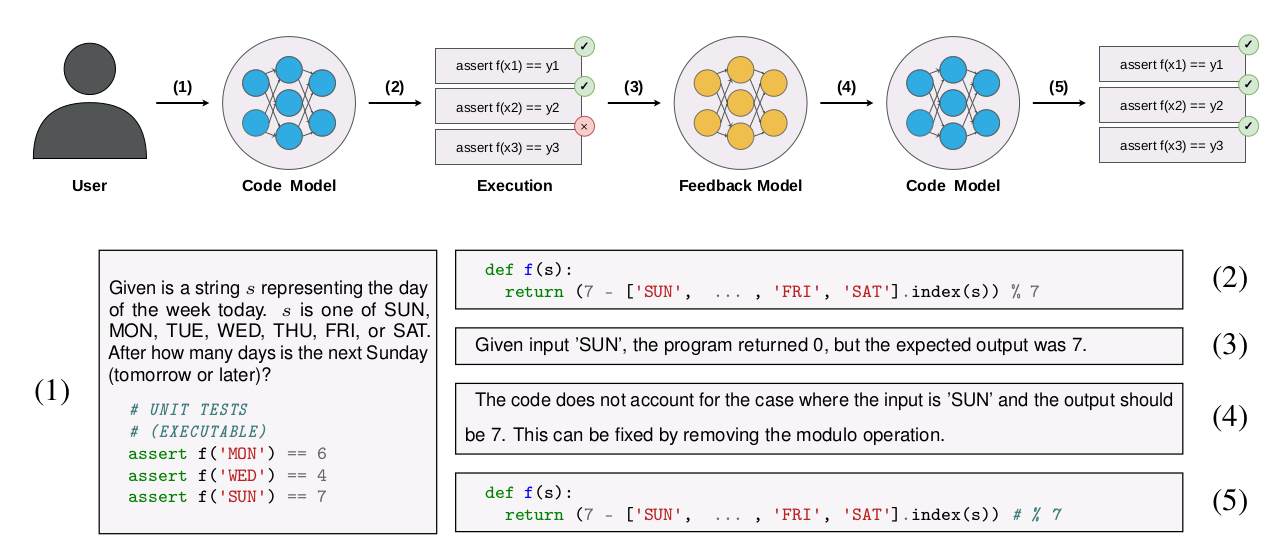
\includegraphics[scale=0.25]{png/example.png}
%     \begin{itemize}
%         \item 
%     \end{itemize}
% \end{frame}

\begin{frame}
    \frametitle{Tree of Thoughts方法}
    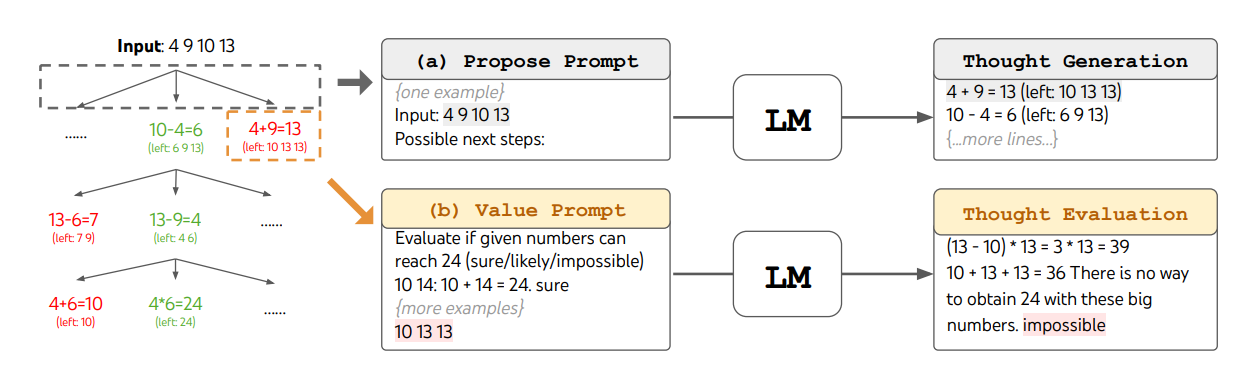
\includegraphics[scale=0.28]{png/process.png}
    \begin{itemize}
        % \item 提出了Tree of Thoughts(ToT)方法:其允许LM通过考虑多种不同的推理路径并且能进行自我评估选择来决定下一步行动,并在必要时looking ahead或回溯以做出全局选择(可以用dfs或者bfs等方法做全局探索),从而进行深思熟虑的决策
        % \item 主要通过Thought decomposition【thought分解】,Thought generator【thought生成】,State evaluator【状态评估】,Search algorithm【搜索算法】四个步骤完成,详情如下
        \item 用一个算24点的例子,来说明具体使用思维树.\\
        \eee{
            \item 思维分解:问题的提问方式可能一样(都是一句话),但是问题类型可以进行细分,比如算24点就是运算一行方程.
            \item 思维生成:生成多种可能,比如像上图中的多行thoughts.
            \item 思维评估:对生成的thoughts进行可能性分析.
            \item 搜索算法:选择合适的算法进行最优结果的搜索.比如这里选择BFS.
        }
    \end{itemize}
\end{frame}

\begin{frame}
    \frametitle{思维树的来源}
    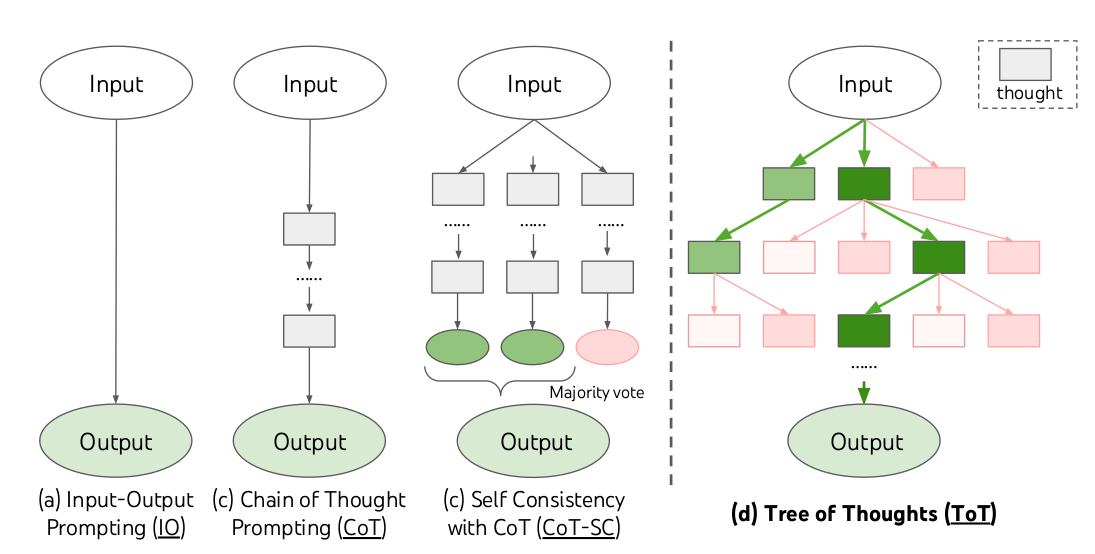
\includegraphics[scale=0.25]{png/tot.png}
    \begin{itemize}
        \item 简单输入输出.
        \item 除了输入输出以外,添加了中间步骤,以及在此基础上加了一些变式.
        \item 将中间步骤变成一种思维树的形式.
    \end{itemize}
\end{frame}

\begin{frame}
    \frametitle{具体的中间步骤解释}
    \begin{itemize}
        \item steps 
        \begin{itemize}
            \item  
            step:0 \\
            "x":"4 5 6 10"\\
            "ys":"之前有的组合" \\
            "new\_ys":"新生成的组合" \\ 
            "values":"计算新生成的组合中评估值"\\
            "select\_new\_ys":"取values最高的5个作为下一步的ys"
            \item  \ff{\vdots}
            \item  
            step:3 \\
            "x":"4 5 6 10"\\
            "ys":"可能的组合" \\
            "new\_ys":"新生成的组合" \\ 
            "values":"计算新生成的组合中评估值"\\
            "select\_new\_ys":"取values最高的5个作为下一步的ys"            
        \end{itemize}
    \end{itemize}
\end{frame}



\begin{frame}
    \frametitle{将现有的输出改成特殊提示的输出}
    \begin{itemize}
        \item  原来的输入,输出
        \eee{
            \item input:预测长度为n的序列\ff{{x_n}}后m结果?
            \item output:\ff{x_{n+1},...,x_{n+m}}
        }
        \item  修改后的输入,输出
        \eee{
            \item input:预测长度为n的序列\ff{{x_n}}后m结果?
            \item output:\\
            step1:\ff{x_{n-m},...,x_{n+1}}\\
            \ff{\vdots} \\
            step(m-1):\ff{x_{n},...,x_{n+m-1}}\\
            step(m):\ff{x_{n+1},...,x_{n+m}}\\a
        }
    \end{itemize}
\end{frame}

\section{代码调试}

\subsection{使用特殊的提示的结果}

\begin{frame}
    \frametitle{\small 使用chatglm2其他提示的见过和没见过任务上的测试1}
	\begin{itemize}
        \item 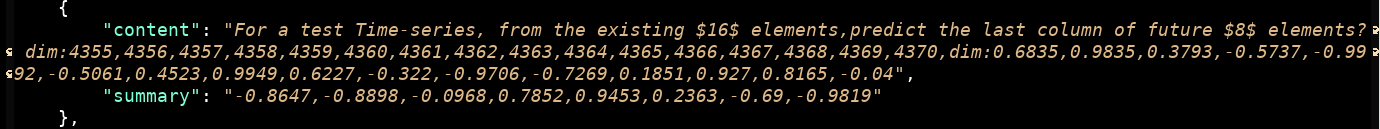
\includegraphics[scale=0.2]{png/prompt1.png}		
        \item 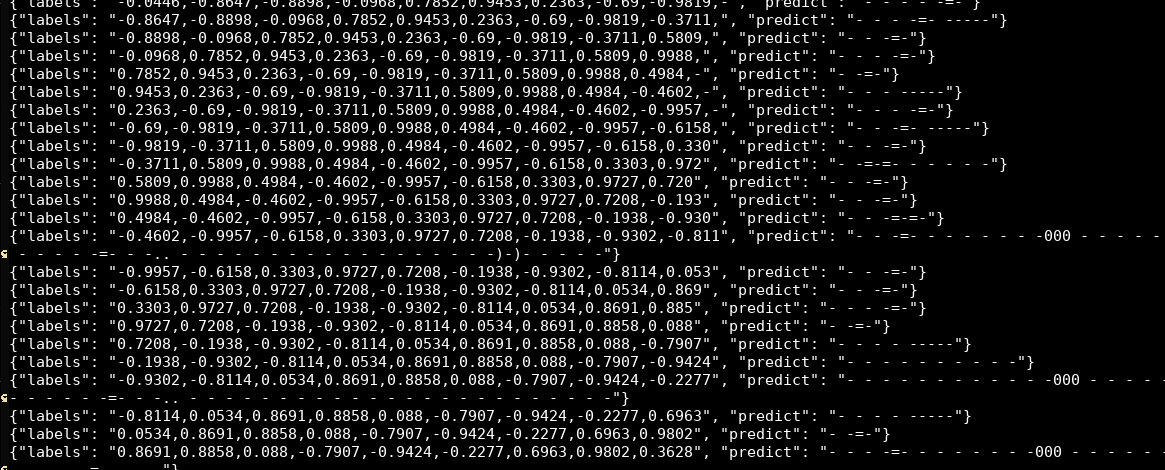
\includegraphics[scale=0.21]{png/error3.png}
        \item 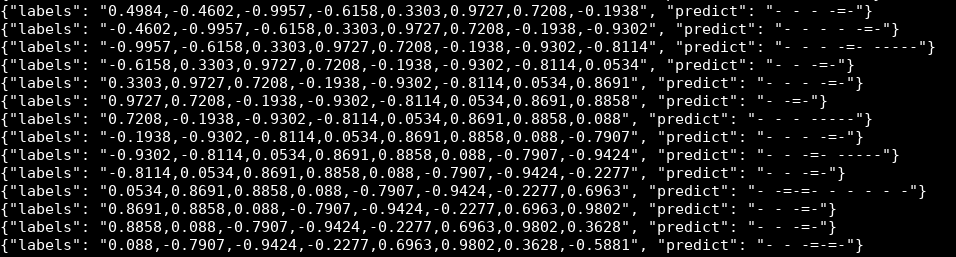
\includegraphics[scale=0.27]{png/error4.png}
	\end{itemize}
\end{frame}

\begin{frame}
    \frametitle{\small 使用chatglm2其他提示的见过和没见过任务上的测试2}
	\begin{itemize}
        \item 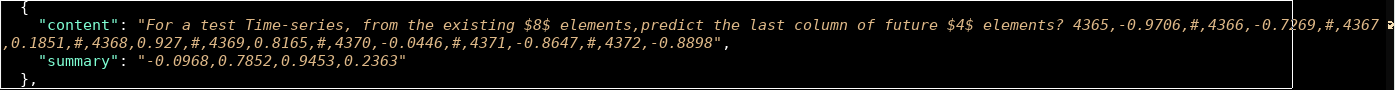
\includegraphics[scale=0.2]{png/prompt2.png}
        \item 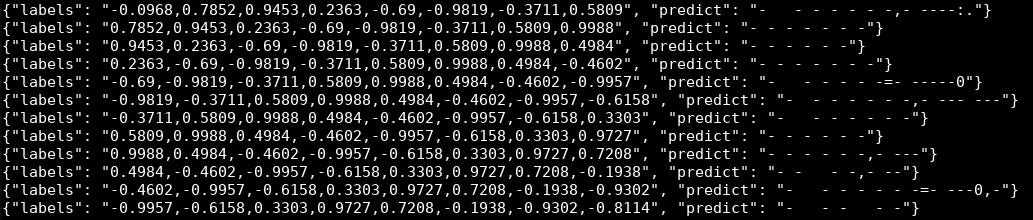
\includegraphics[scale=0.24]{png/error5.png}
        \item 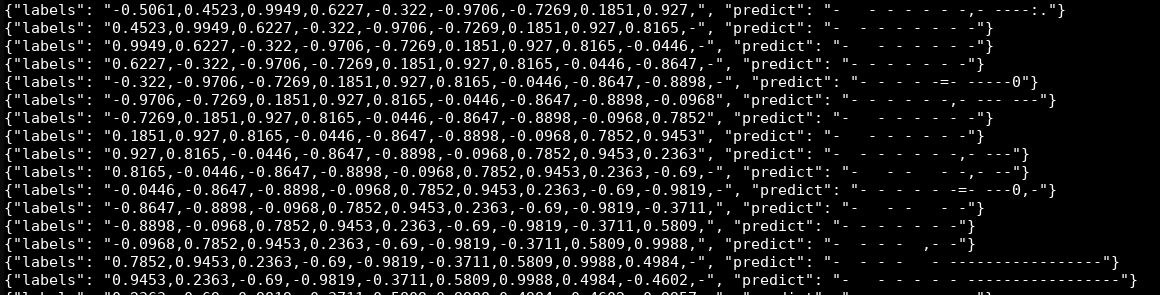
\includegraphics[scale=0.23]{png/error6.png}
	\end{itemize}
\end{frame}


\subsection{添加中间步骤的输出后的结果}

\begin{frame}
    \frametitle{添加部分步骤的提示结果}  
	\begin{itemize}
        \item 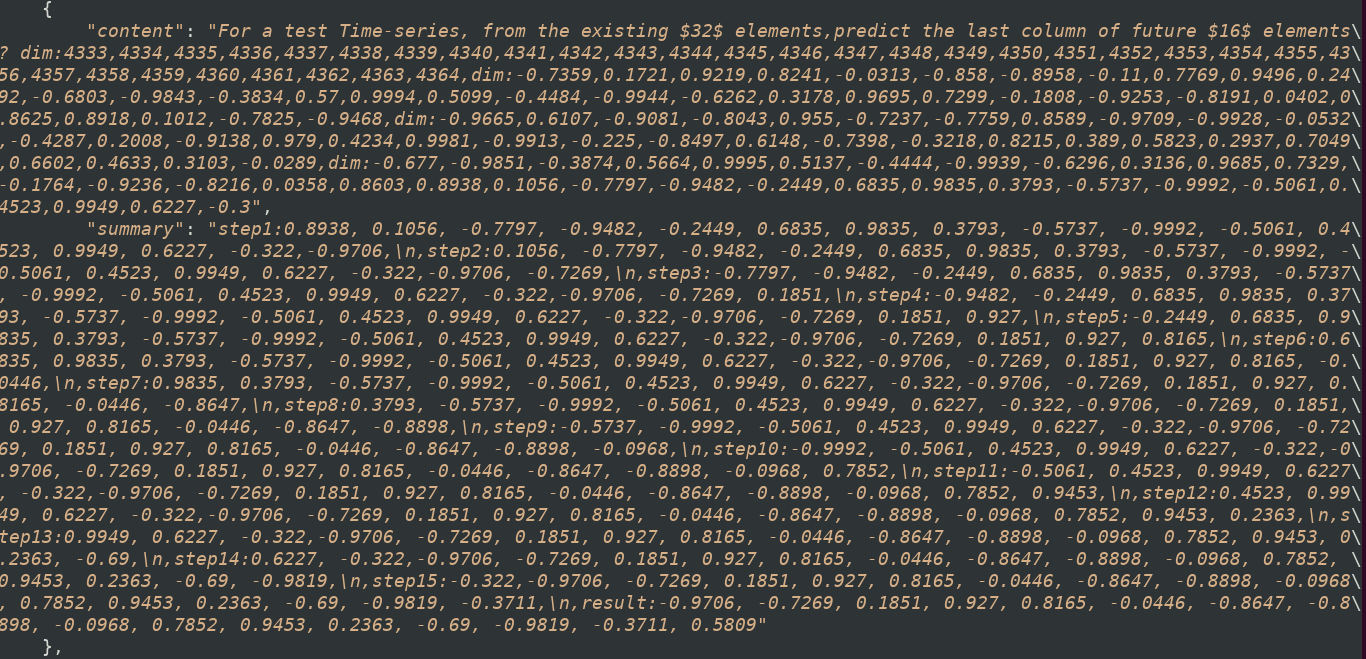
\includegraphics[scale=0.2]{png/prompt3.png}
		\item 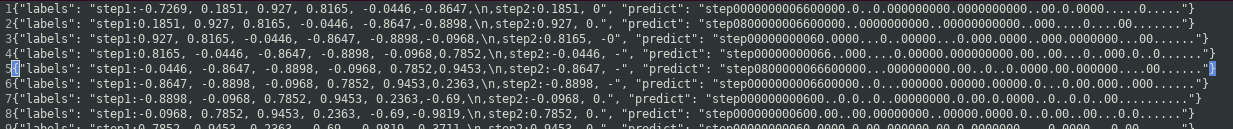
\includegraphics[scale=0.2555]{png/error7.png}
	\end{itemize}
\end{frame}




% \begin{frame}
%     \frametitle{ new prompt(泛化性能测试)}  
% 	\begin{itemize}
% 		\item 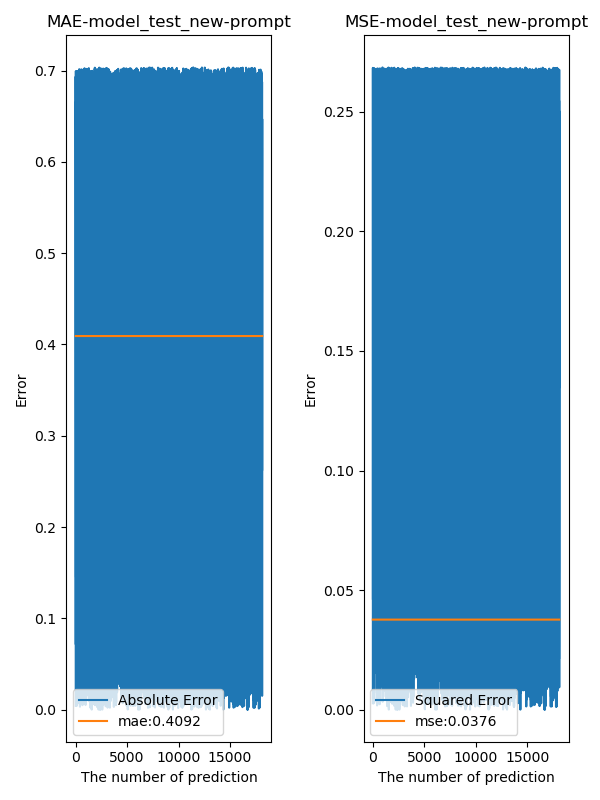
\includegraphics[scale=0.3555]{png/model_test_new-prompt.png}
% 	\end{itemize}
% \end{frame}

% \begin{frame}
%     \frametitle{ old prompt(泛化性能测试)}  
% 	\begin{itemize}
% 		\item 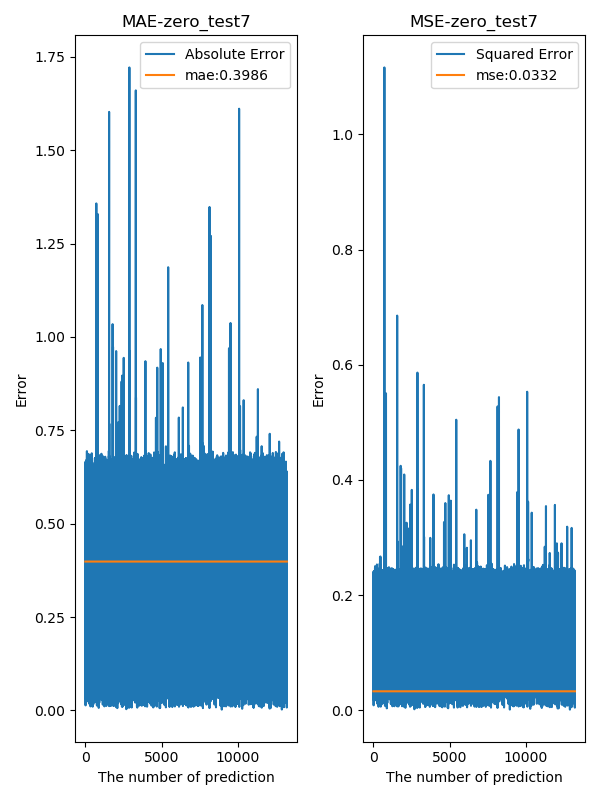
\includegraphics[scale=0.3555]{png/zero_test7.png}
% 	\end{itemize}
% \end{frame}


% \begin{frame}
% 	% \frametitle{\tiny 准确率:66.95\%,使用具有zero\_model\_test去预测mix\_5000\_16-80-4\_2-function中的内容}
%     \frametitle{\tiny 训练总数据量:640000,预测长度:8预测4,...,80预测40,间隔4;用于训练的函数序列:8种基本函数,如三角,多项式函数,对数,平方根等 \\
%     待预测的数据:16预测8,...,80预测40,间隔为4;预测的函数序列:2种不同的函数序列;准确率:66.95\%} 
%     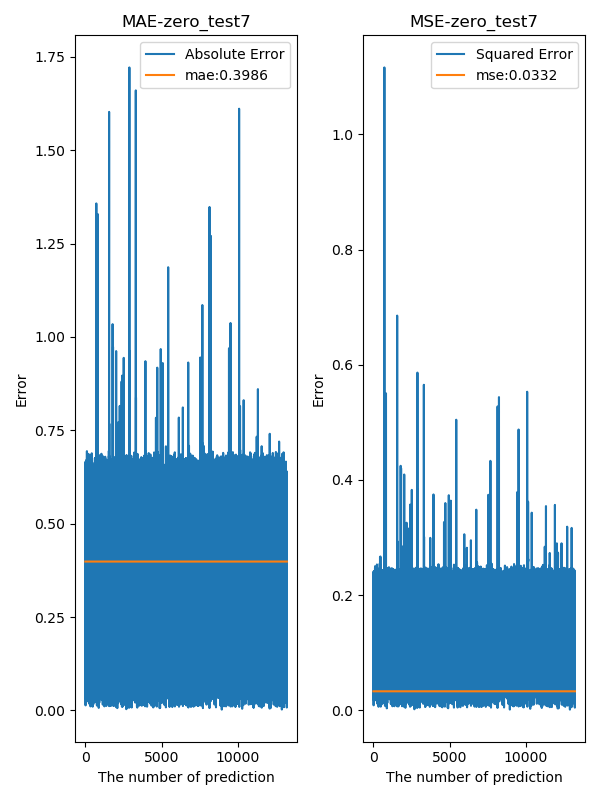
\includegraphics[scale=0.3555]{png/zero_test7.png}
% 	% \begin{itemize}
% 		%	\item 是否一个更加综合的模型能够对结果有更强的泛化能力?
% 	% \end{itemize}
% \end{frame}


% \begin{frame}
% 	\frametitle{\small 总数据量:30000,16预测8,长向量序列预测}	
% 	\begin{itemize}
% 		% \item 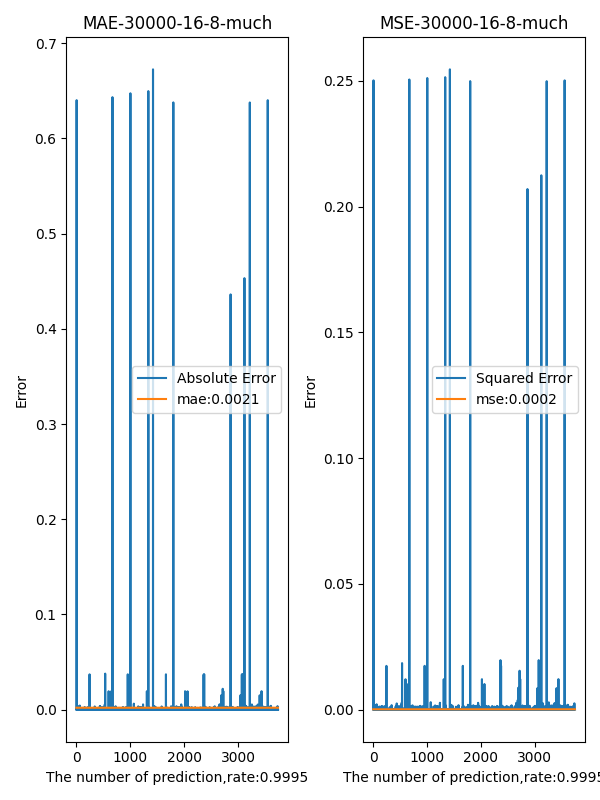
\includegraphics[scale=0.3555]{png/30000-16-8-much.png}
% 	\end{itemize}
% \end{frame}

\subsection{实验结果分析}
\begin{frame}
	\frametitle{实验结论}	
	\begin{itemize}
        % \item 这个到底是什么原因啊?为啥这个不一样啊.
        \item chatglm2的训练结果不如chatglm.之后测试可能还需要用chatglm来做
        \item 可能是因为
        % \item 使用新的提示后,部分测试结果出现了乱码现象.
        % \eee{
        %     \item 使用chatglm2训练一个大型数据集合时,在预测已经见过的任务上出现了乱码的现象.
        %     \item 使用chatglm进行泛化测试的一个实验,也出现了乱码的情况.
        % }
	\end{itemize}
\end{frame}

% \subsection{实验过程中遇到的一些问题}

% \begin{frame}
% 	\frametitle{遇到的问题}	
% 	\begin{itemize}
%         \item 目标预测的个数和实际预测个数不同或者预测非数值形式,下面是一些解决方法
%         \eee{
%             \item 忽略实际预测个数和目标个数不同的例子,并计算其比率rate(目标与实际个数相同的个数/测试集个数)
%             \item 对预测得到的结果进行截断或补零
%         }   
%         \item 序列长度太长的问题
% 	\end{itemize}
%     % 目前考虑的是只考虑数量对等的
% \end{frame}


\subsection{下一步的计划}
\begin{frame}
	\frametitle{下一步计划}	
	\begin{itemize}
        % \item 是否还要使用新的提示方式?(可能更加简洁的提示效果会更好)
        \item 部署llama2,使其能够像chatglm一样进行类似训练和评估.
        \item 通过其他方式在chatglm上添加中间步骤看看效果如何?
        \item 提高模型的泛化能力
        \eee{
            % \item 在通过修改提示的方式上目前效果不太好.
            \item 添加思维树的方式来提高泛化能力
            % \item 
        }
	\end{itemize}
\end{frame}

% 结束语
\section{}
\begin{frame}
	\frametitle{}
	\begin{center}
		\Huge{谢谢老师和同学们的聆听!}
	\end{center}
\end{frame}

\end{CJK*}
\end{document}